\href{https://github.com/yassienE4/OS-VM/commit/6cb8e1e5887e13f7748f728cdeeb3f62c72b3c69}{\ul{https://github.com/yassienE4/OS-VM/commit/6cb8e1e5887e13f7748f728cdeeb3f62c72b3c69}}

How to run

\begin{itemize}
\item
  First move to working directory
\item
  cd chat
\item
  Compile both server and client
\item
  g++ server.cpp -o server -pthread
\item
  g++ client.cpp -o client -pthread
\item
  ./server
\item
  Then instantiate as many clients as needed
\item
  ./client
\end{itemize}

Server

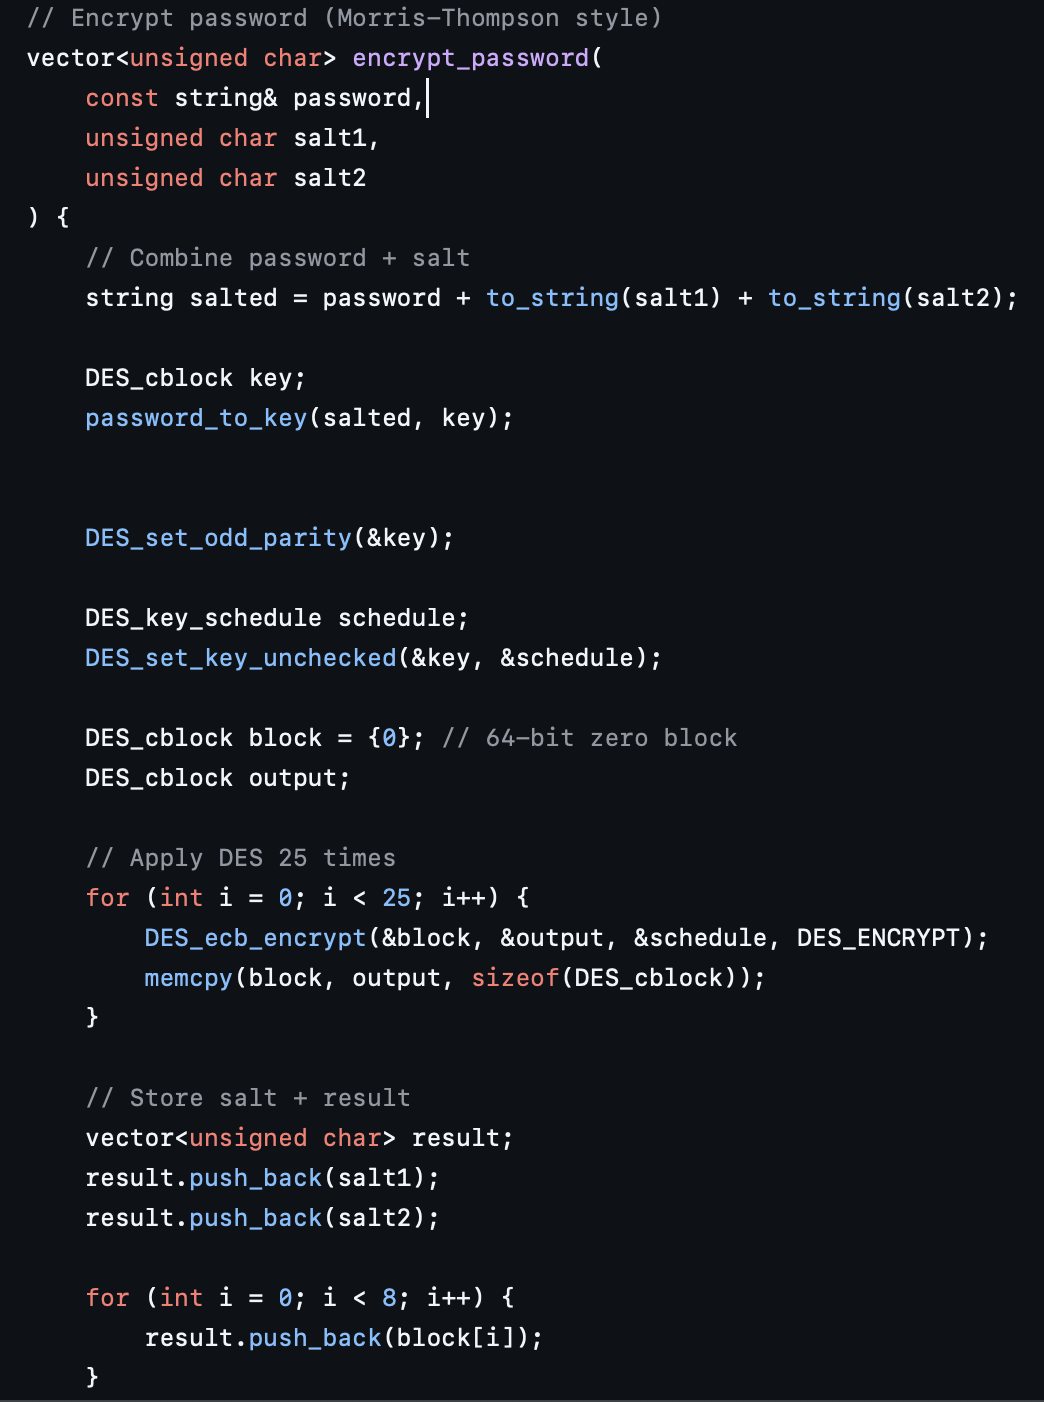
\includegraphics[width=6.5in,height=4.09722in]{./images/media/image4.png}

First we init a socket, and set the server to listening mode, while
consistently receiving sockets from potential clients, then we handle
the client in a separate thread so that messages are received
asynchronously

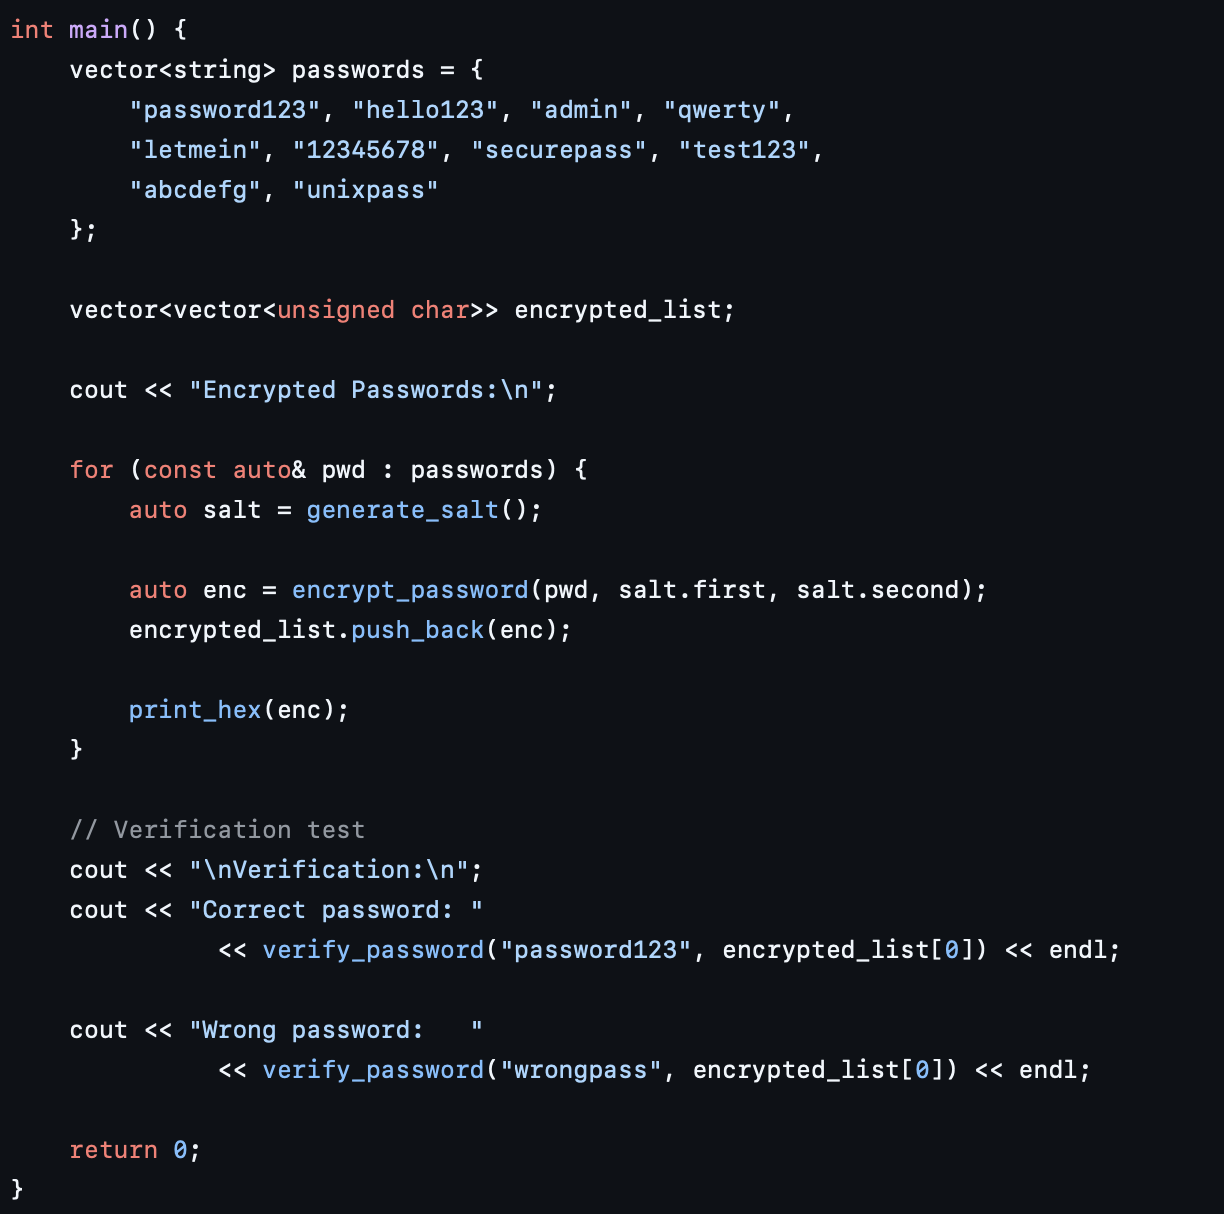
\includegraphics[width=6.5in,height=6.02778in]{./images/media/image3.png}

Here we just format the message and broadcast it

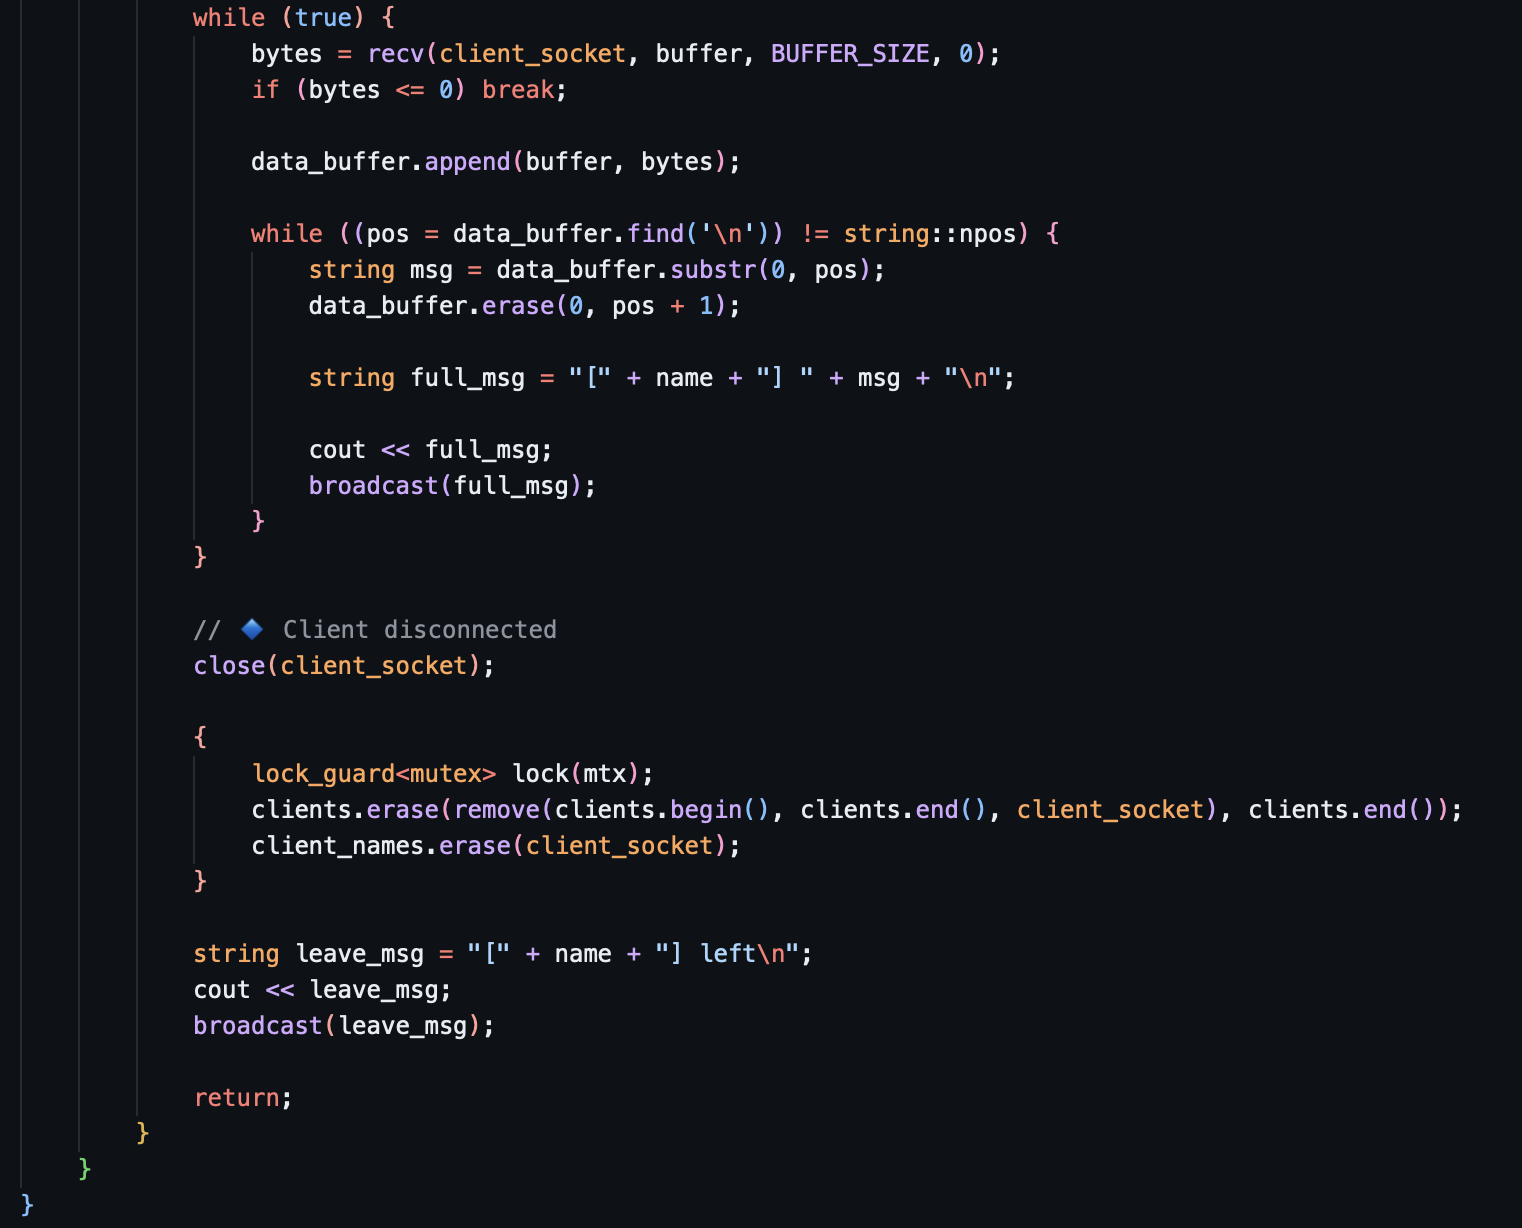
\includegraphics[width=6.5in,height=5.25in]{./images/media/image6.png}

Here we disconnect the client

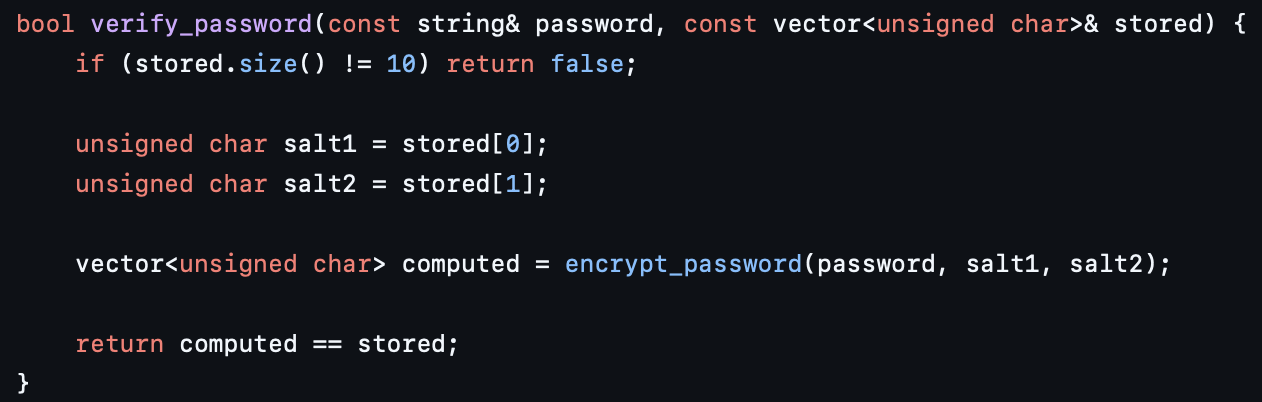
\includegraphics[width=6.5in,height=3.11111in]{./images/media/image2.png}

This broadcasts the messages to potential servers

Client

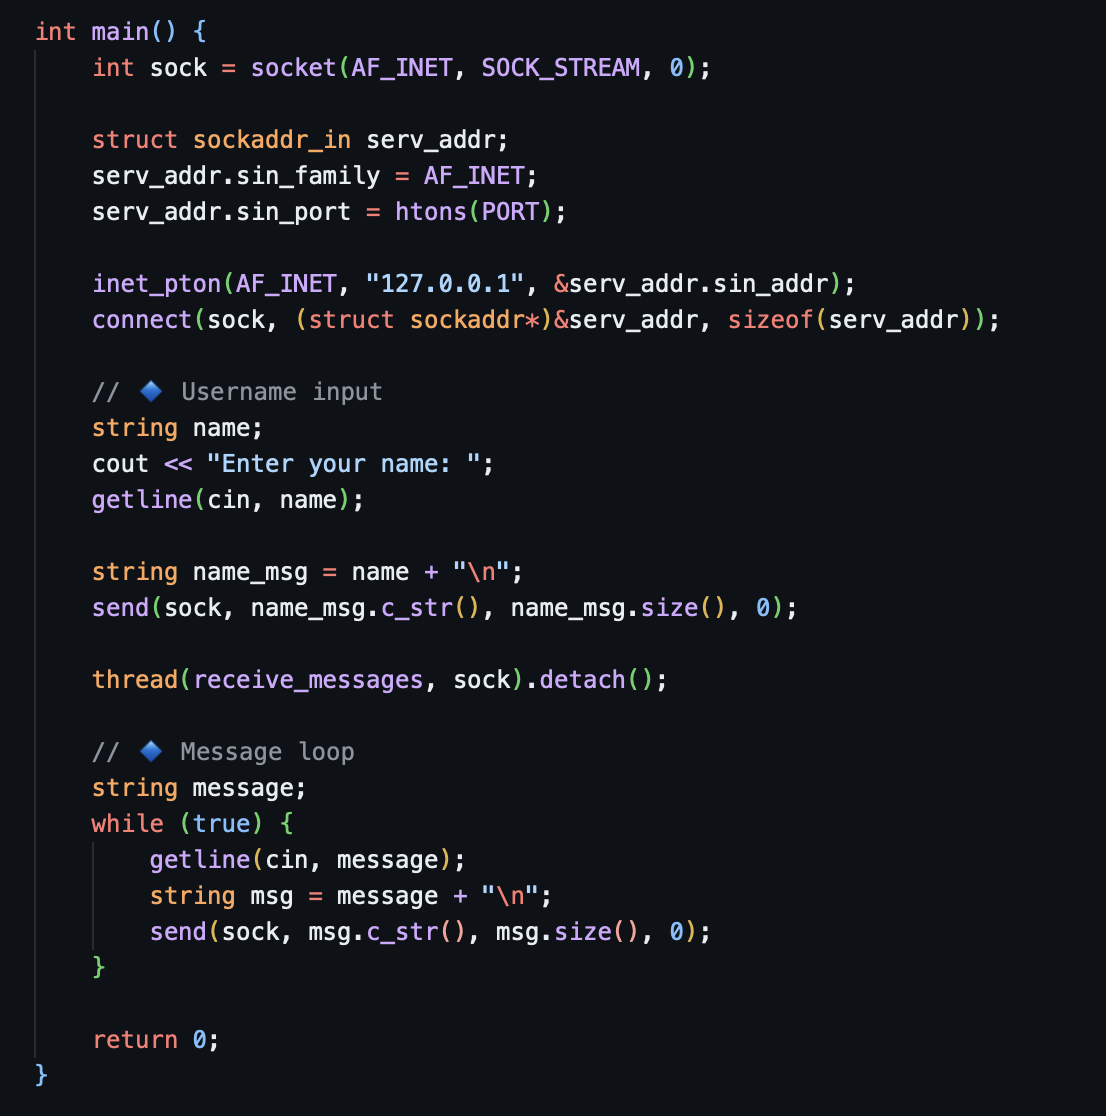
\includegraphics[width=6.5in,height=6.55556in]{./images/media/image5.png}

Similarly to the server we create a socket then set it to connect to the
server

We then receive a username and create messages using it

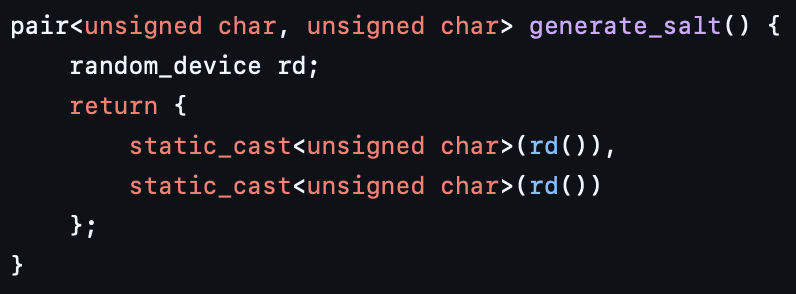
\includegraphics[width=6.5in,height=5.27778in]{./images/media/image1.png}

To receive messages as a client we just decode the buffer and format it
